% Options for packages loaded elsewhere
\PassOptionsToPackage{unicode,colorlinks=true,linkcolor=blue,urlcolor=cyan}{hyperref}
\PassOptionsToPackage{hyphens}{url}
\PassOptionsToPackage{dvipsnames,svgnames,x11names}{xcolor}
%
\documentclass[
  openany]{scrbook}

\usepackage{amsmath,amssymb}
\usepackage{lmodern}
\usepackage{iftex}
\ifPDFTeX
  \usepackage[T1]{fontenc}
  \usepackage[utf8]{inputenc}
  \usepackage{textcomp} % provide euro and other symbols
\else % if luatex or xetex
  \usepackage{unicode-math}
  \defaultfontfeatures{Scale=MatchLowercase}
  \defaultfontfeatures[\rmfamily]{Ligatures=TeX,Scale=1}
\fi
% Use upquote if available, for straight quotes in verbatim environments
\IfFileExists{upquote.sty}{\usepackage{upquote}}{}
\IfFileExists{microtype.sty}{% use microtype if available
  \usepackage[]{microtype}
  \UseMicrotypeSet[protrusion]{basicmath} % disable protrusion for tt fonts
}{}
\makeatletter
\@ifundefined{KOMAClassName}{% if non-KOMA class
  \IfFileExists{parskip.sty}{%
    \usepackage{parskip}
  }{% else
    \setlength{\parindent}{0pt}
    \setlength{\parskip}{6pt plus 2pt minus 1pt}}
}{% if KOMA class
  \KOMAoptions{parskip=half}}
\makeatother
\usepackage{xcolor}
\usepackage[margin=1.5in]{geometry}
\setlength{\emergencystretch}{3em} % prevent overfull lines
\setcounter{secnumdepth}{5}
% Make \paragraph and \subparagraph free-standing
\ifx\paragraph\undefined\else
  \let\oldparagraph\paragraph
  \renewcommand{\paragraph}[1]{\oldparagraph{#1}\mbox{}}
\fi
\ifx\subparagraph\undefined\else
  \let\oldsubparagraph\subparagraph
  \renewcommand{\subparagraph}[1]{\oldsubparagraph{#1}\mbox{}}
\fi


\providecommand{\tightlist}{%
  \setlength{\itemsep}{0pt}\setlength{\parskip}{0pt}}\usepackage{longtable,booktabs,array}
\usepackage{calc} % for calculating minipage widths
% Correct order of tables after \paragraph or \subparagraph
\usepackage{etoolbox}
\makeatletter
\patchcmd\longtable{\par}{\if@noskipsec\mbox{}\fi\par}{}{}
\makeatother
% Allow footnotes in longtable head/foot
\IfFileExists{footnotehyper.sty}{\usepackage{footnotehyper}}{\usepackage{footnote}}
\makesavenoteenv{longtable}
\usepackage{graphicx}
\makeatletter
\def\maxwidth{\ifdim\Gin@nat@width>\linewidth\linewidth\else\Gin@nat@width\fi}
\def\maxheight{\ifdim\Gin@nat@height>\textheight\textheight\else\Gin@nat@height\fi}
\makeatother
% Scale images if necessary, so that they will not overflow the page
% margins by default, and it is still possible to overwrite the defaults
% using explicit options in \includegraphics[width, height, ...]{}
\setkeys{Gin}{width=\maxwidth,height=\maxheight,keepaspectratio}
% Set default figure placement to htbp
\makeatletter
\def\fps@figure{htbp}
\makeatother
\newlength{\cslhangindent}
\setlength{\cslhangindent}{1.5em}
\newlength{\csllabelwidth}
\setlength{\csllabelwidth}{3em}
\newlength{\cslentryspacingunit} % times entry-spacing
\setlength{\cslentryspacingunit}{\parskip}
\newenvironment{CSLReferences}[2] % #1 hanging-ident, #2 entry spacing
 {% don't indent paragraphs
  \setlength{\parindent}{0pt}
  % turn on hanging indent if param 1 is 1
  \ifodd #1
  \let\oldpar\par
  \def\par{\hangindent=\cslhangindent\oldpar}
  \fi
  % set entry spacing
  \setlength{\parskip}{#2\cslentryspacingunit}
 }%
 {}
\usepackage{calc}
\newcommand{\CSLBlock}[1]{#1\hfill\break}
\newcommand{\CSLLeftMargin}[1]{\parbox[t]{\csllabelwidth}{#1}}
\newcommand{\CSLRightInline}[1]{\parbox[t]{\linewidth - \csllabelwidth}{#1}\break}
\newcommand{\CSLIndent}[1]{\hspace{\cslhangindent}#1}

\usepackage{hyphenat}
\usepackage{graphicx}
\usepackage{geometry}
\usepackage{afterpage}
\usepackage{tikz}
\usetikzlibrary{fadings}
\usepackage[pagecolor=none]{pagecolor}







\makeatletter
\makeatother
\makeatletter
\makeatother
\makeatletter
\@ifpackageloaded{caption}{}{\usepackage{caption}}
\AtBeginDocument{%
\ifdefined\contentsname
  \renewcommand*\contentsname{Table of contents}
\else
  \newcommand\contentsname{Table of contents}
\fi
\ifdefined\listfigurename
  \renewcommand*\listfigurename{List of Figures}
\else
  \newcommand\listfigurename{List of Figures}
\fi
\ifdefined\listtablename
  \renewcommand*\listtablename{List of Tables}
\else
  \newcommand\listtablename{List of Tables}
\fi
\ifdefined\figurename
  \renewcommand*\figurename{Figure}
\else
  \newcommand\figurename{Figure}
\fi
\ifdefined\tablename
  \renewcommand*\tablename{Table}
\else
  \newcommand\tablename{Table}
\fi
}
\@ifpackageloaded{float}{}{\usepackage{float}}
\floatstyle{ruled}
\@ifundefined{c@chapter}{\newfloat{codelisting}{h}{lop}}{\newfloat{codelisting}{h}{lop}[chapter]}
\floatname{codelisting}{Listing}
\newcommand*\listoflistings{\listof{codelisting}{List of Listings}}
\makeatother
\makeatletter
\@ifpackageloaded{caption}{}{\usepackage{caption}}
\@ifpackageloaded{subcaption}{}{\usepackage{subcaption}}
\makeatother
\makeatletter
\@ifpackageloaded{tcolorbox}{}{\usepackage[many]{tcolorbox}}
\makeatother
\makeatletter
\@ifundefined{shadecolor}{\definecolor{shadecolor}{rgb}{.97, .97, .97}}
\makeatother
\makeatletter
\makeatother
\ifLuaTeX
  \usepackage{selnolig}  % disable illegal ligatures
\fi
\IfFileExists{bookmark.sty}{\usepackage{bookmark}}{\usepackage{hyperref}}
\IfFileExists{xurl.sty}{\usepackage{xurl}}{} % add URL line breaks if available
\urlstyle{same} % disable monospaced font for URLs
\hypersetup{
  pdftitle={quarto\_titlepages},
  pdfauthor={Elizabeth Eli Holmes},
  colorlinks=true,
  linkcolor={blue},
  filecolor={Maroon},
  citecolor={Blue},
  urlcolor={cyan},
  pdfcreator={LaTeX via pandoc}}

\title{quarto\_titlepages}
\usepackage{etoolbox}
\makeatletter
\providecommand{\subtitle}[1]{% add subtitle to \maketitle
  \apptocmd{\@title}{\par {\large #1 \par}}{}{}
}
\makeatother
\subtitle{Templates for title pages and covers}
\author{Elizabeth Eli Holmes}
\date{}

\begin{document}
\begin{frontmatter}
\begin{titlepage}
% This is a combination of Pandoc templating and LaTeX
% Pandoc templating https://pandoc.org/MANUAL.html#templates
% See the README for help
% This template is based on a post by Arun Debray to tex.stackoverflow
% https://tex.stackexchange.com/posts/554962/revisions

\newgeometry{left=1in, right=1in,top=2in, bottom=0in}
\begin{minipage}[b][\textheight][s]{\textwidth}

% Change title fonts here
\DeclareFixedFont{\titlefont}{T1}{ppl}{b}{}{0.6in}
\DeclareFixedFont{\subtitlefont}{T1}{ppl}{b}{it}{0.2in}

% Page color
\definecolor{pgcolor}{HTML}{F6D5A8}
\pagecolor{pgcolor}\afterpage{\nopagecolor}

\thispagestyle{empty}
\begin{flushright}
\titlefont quarto\_titlepages\\
\subtitlefont Templates for title pages and covers
\end{flushright}
\vfill
\begin{center}
\begin{tikzpicture}
\node[scope fading=north, inner sep=0pt, outer sep=0pt]{
 \makebox[\textwidth]{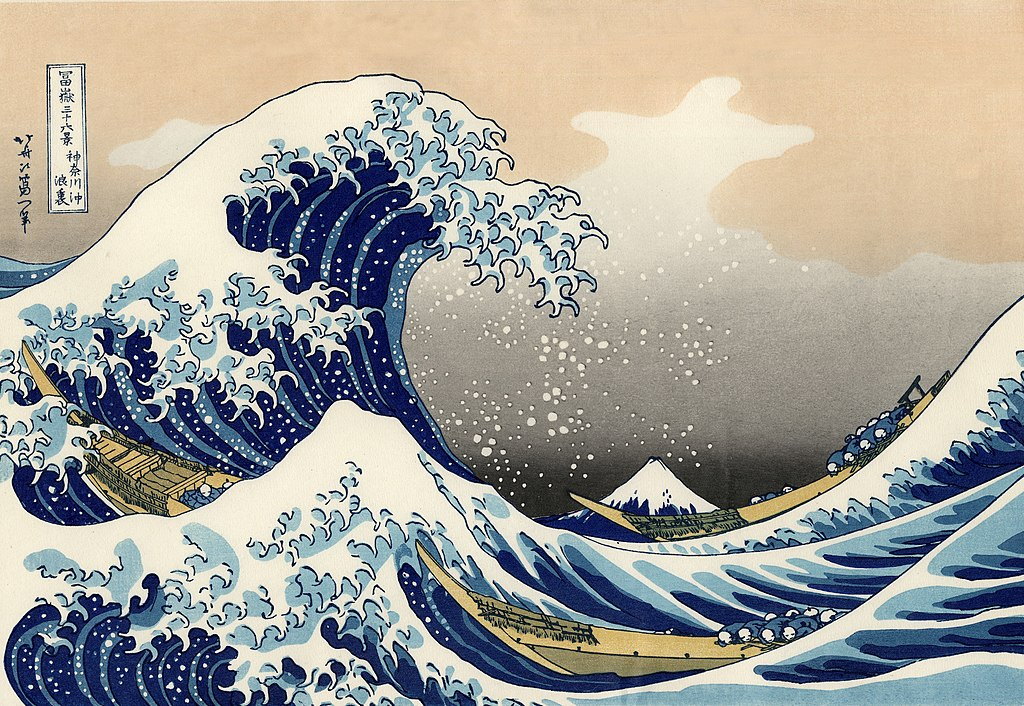
\includegraphics[width=\paperwidth]{images/TheGreatWaveoffKanagawa.jpeg}}
};
\end{tikzpicture}
\end{center}

\end{minipage}%
\clearpage
\restoregeometry%
% for some reason it insists on putting a black page
% between cover and title if I have this above \begin{titlepage}
% This is a combination of Pandoc templating and LaTeX
% Pandoc templating https://pandoc.org/MANUAL.html#templates
% See the README for help

\raggedleft % left align the title page
\thispagestyle{empty}
\rule{1pt}{\textheight} % Vertical line
\hspace{0.05\textwidth} % Whitespace between the vertical line and title page text
% Adjust num before \textwidth to move the block left or right
\begin{minipage}[b][\textheight][s]{0.85\textwidth}

\raggedright
% Title and subtitle
{\huge\bfseries\nohyphens{quarto\_titlepages}}\\[1.25\baselineskip] 
{\large\textit{Templates for title pages and covers}}\\[4\baselineskip]

% Abstract
%
\begin{flushright}%
{{\href{https://nmfs-opensci.github.io/quarto_titlepages}{quarto\_titlepages}:
GitHub repo with template partials for use with
\href{https://quarto.org/}{Quarto} for adding custom cover pages and
title pages to your PDF books or articles. Documentation included for
using the provided templates or modifying to create your
own.}}\\[4\baselineskip]%
\end{flushright}%


% Authors	
% This hairy bit of code is just to get "and" between the last 2
% authors. See below if you don't need that
%
{\large{Elizabeth Eli Holmes}}%
%
{\textsuperscript{1}}\textsuperscript{,}%
{\textsuperscript{2}}%
%
\textsuperscript{,}%
{\textsuperscript{,*}}%
%


% This is how to do it if you don't need the "and"


%%%%%% Affiliations
\vspace{2\baselineskip} 

\hangindent=1em
\hangafter=1
%
{1}.~{NOAA Fisheries}%
%
%
, %
{Northwest Fisheries Science Center, Seattle WA, USA}%
%
\par\hangindent=1em\hangafter=1%
%
{2}.~{University of Washington}%
%
, %
{School of Aquatic and Fishery Sciences}%
%
%


%%%%%% Correspondence
\vspace{1\baselineskip} 

* \textit{Correspondence:}~Elizabeth Eli Holmes~eli.holmes@noaa.gov

%use \vfill instead to get the space to fill flexibly	
%\vspace{0.25\textheight} % Whitespace between the title block and the publisher

\vfill

%%%%%% Cover image

\includegraphics[width=4cm]{images/nmfs-opensci-logo.png}

% Whitespace between the title block and the tagline
\vspace{0.1\textheight} 

%%%%%% Tagline at bottom
{\noindent https://nmfs-opensci.github.io/}\\[\baselineskip]
\end{minipage}  
\end{titlepage}
\setcounter{page}{1}
\end{frontmatter}

  \ifdefined\Shaded\renewenvironment{Shaded}{\begin{tcolorbox}[interior hidden, breakable, boxrule=0pt, sharp corners, borderline west={3pt}{0pt}{shadecolor}, frame hidden, enhanced]}{\end{tcolorbox}}\fi

\renewcommand*\contentsname{Table of contents}
{
\hypersetup{linkcolor=}
\setcounter{tocdepth}{2}
\tableofcontents
}
\listoffigures
\listoftables
\mainmatter
\hypertarget{notes-on-great-wave}{%
\chapter{Notes on great-wave}\label{notes-on-great-wave}}

\begin{itemize}
\tightlist
\item
  classoptions \texttt{openany} (allows chapters to start on even or odd
  pages) and \texttt{onepage} (same margins on even and odd pages) do
  not work together. If you set \texttt{openany}, then \texttt{onepage}
  is ignored. So set \texttt{openany} as class option and then set
  geometry so that all pages have the same geometry (meaning margins).
  The code in \texttt{\_coverpage.tex} will set its own geometry for the
  cover page.
\item
  filenames with \texttt{\_} don't work across all operating systems. I
  always forget what symbols are bad in what operating system so I try
  to have no symbols in included image file names.
\item
  Use \texttt{titlepage-geometry:} to move your title around so it
  doesn't overlap your image.
\item
  Use \texttt{titlepage-color} to get a background color that matches
  the image and gets a nice fade.
\end{itemize}

\hypertarget{introduction}{%
\chapter{Introduction}\label{introduction}}

Lorem ipsum dolor sit amet, consectetur adipiscing elit. Proin eu tempor
velit. Fusce accumsan ultrices fringilla. Praesent sed odio mi. Mauris
non ligula turpis. Duis posuere lacus nec diam interdum dictum suscipit
magna molestie. Vestibulum nibh dolor, interdum eget rhoncus ut, sodales
eget justo. Morbi blandit lorem sit amet nulla egestas aliquam. Nunc
pharetra est at nibh ullamcorper in commodo erat dignissim. Cras et
suscipit enim.

Lorem ipsum dolor sit amet, consectetur adipiscing elit. Phasellus neque
ex, vehicula dictum risus fermentum, feugiat faucibus neque. Etiam purus
quam, lacinia vel porta in, malesuada ac nisl. Vestibulum ante ipsum
primis in faucibus orci luctus et ultrices posuere cubilia curae; Sed
bibendum placerat tellus, ac finibus lectus euismod eget.

Nulla mattis diam vitae bibendum consequat. Etiam vitae eros tristique,
porta sapien a, aliquet mauris. Praesent ultricies mi nulla, et
dignissim nulla mattis at. Fusce rhoncus leo quis odio euismod,
hendrerit facilisis risus tincidunt. Aenean at lectus justo. Cras
fringilla lacus nisl, ac convallis odio tincidunt vel. Integer vel
egestas nisi. Curabitur vitae imperdiet justo.

\begin{quote}
Lorem ipsum dolor sit amet, consectetur adipiscing elit, sed do eiusmod
tempor incididunt ut labore et dolore magna aliqua. Ut enim ad minim
veniam, quis nostrud exercitation ullamco laboris nisi ut aliquip ex ea
commodo consequat.\\
\end{quote}

\hypertarget{supporting-theory}{%
\section{Supporting theory}\label{supporting-theory}}

Let \(X_1, X_2, \ldots, X_n\) be a sequence of independent and
identically distributed random variables with \(\text{E}[X_i] = \mu\)
and \(\text{Var}[X_i] = \sigma^2 < \infty\), and let

\begin{equation}\protect\hypertarget{eq-clt}{}{
S_n = \frac{X_1 + X_2 + \cdots + X_n}{n}
      = \frac{1}{n}\sum_{i}^{n} X_i
}\label{eq-clt}\end{equation}

denote their mean. Then as \(n\) approaches infinity, the random
variables \(\sqrt{n}(S_n - \mu)\) converge in distribution to a normal
\(\mathcal{N}(0, \sigma^2)\). Thus concludes the explanation about
Equation~\ref{eq-clt}.

\hypertarget{materials-and-methods}{%
\chapter{Materials and Methods}\label{materials-and-methods}}

Lorem ipsum dolor sit amet, consectetur adipiscing elit. Phasellus neque
ex, vehicula dictum risus fermentum, feugiat faucibus neque. Etiam purus
quam, lacinia vel porta in, malesuada ac nisl. Vestibulum ante ipsum
primis in faucibus orci luctus et ultrices posuere cubilia curae; Sed
bibendum placerat tellus, ac finibus lectus euismod eget.

\hypertarget{study-area}{%
\section{Study area}\label{study-area}}

Lorem ipsum dolor sit amet, consectetur adipiscing elit. Phasellus neque
ex, vehicula dictum risus fermentum, feugiat faucibus neque. Etiam purus
quam, lacinia vel porta in, malesuada ac nisl. Vestibulum ante ipsum
primis in faucibus orci luctus et ultrices posuere cubilia curae; Sed
bibendum placerat tellus, ac finibus lectus euismod eget. Nulla mattis
diam vitae bibendum consequat.

\begin{figure}

{\centering 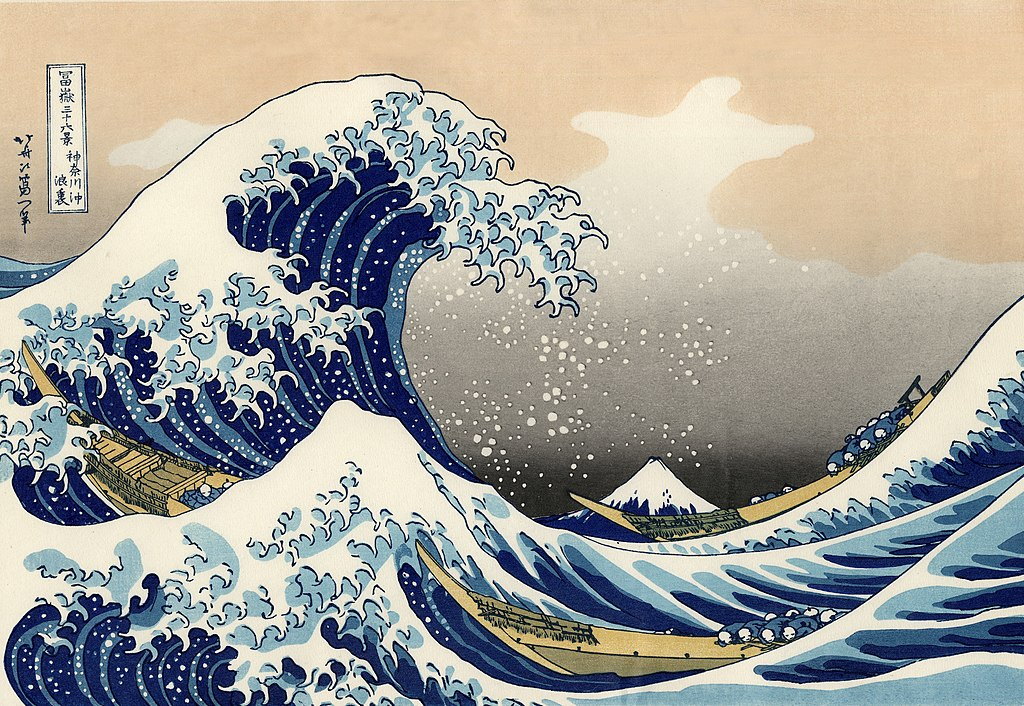
\includegraphics{images/TheGreatWaveoffKanagawa.jpeg}

}

\caption{\label{fig-wave}great wave}

\end{figure}

See Figure~\ref{fig-wave} for a picture of the study animal. Etiam vitae
eros tristique, porta sapien a, aliquet mauris. Praesent ultricies mi
nulla, et dignissim nulla mattis at. Fusce rhoncus leo quis odio
euismod, hendrerit facilisis risus tincidunt. Aenean at lectus justo.
Cras fringilla lacus nisl, ac convallis odio tincidunt vel. Integer vel
egestas nisi. Curabitur vitae imperdiet justo.

Curabitur efficitur in risus quis egestas. Suspendisse porta interdum
leo ac ultricies. Pellentesque bibendum, felis vitae fermentum eleifend,
nunc nunc fermentum nisi, ac maximus felis lacus lobortis risus.
Suspendisse potenti. Nunc vitae consequat elit. Fusce id ligula sed
lectus condimentum laoreet. Vestibulum faucibus commodo suscipit. Nulla
tempor tellus vel massa efficitur euismod. Duis nec commodo mauris, sit
amet tincidunt elit. Cras mollis non ante sed venenatis. In ultricies
ante accumsan lectus rhoncus, vel pharetra sem convallis.

\hypertarget{results}{%
\chapter{Results}\label{results}}

See Table~\ref{tbl-numbers} for the table of results. Phasellus quis
orci nec erat suscipit imperdiet. Aenean pulvinar enim ut ante
convallis, vel sollicitudin purus malesuada. Sed sed ullamcorper urna.
Morbi sed lobortis neque, sit amet hendrerit magna. Donec ultricies
pretium lorem, eget sagittis metus posuere et. Aenean ex purus, aliquam
sit amet tellus ut, pellentesque porttitor orci. Integer quis mi
pharetra, bibendum neque nec, viverra nulla. Cras quis magna in erat
facilisis consequat. Vivamus sed lectus iaculis, euismod ligula eu,
fermentum sem.

\hypertarget{tbl-numbers}{}
\begin{longtable}[]{@{}lr@{}}
\caption{\label{tbl-numbers}Table of numbers.}\tabularnewline
\toprule()
Thing & Value \\
\midrule()
\endfirsthead
\toprule()
Thing & Value \\
\midrule()
\endhead
A 42 & 18 \\
B 15 & 18 \\
C 34 & 17 \\
D 99 & 24 \\
\bottomrule()
\end{longtable}

\hypertarget{discussion}{%
\chapter{Discussion}\label{discussion}}

Lorem ipsum dolor sit amet, Table~\ref{tbl-numbers}, consectetur
adipiscing elit. Knuth (1984) and all things LaTeX. Phasellus neque ex,
vehicula dictum risus fermentum, feugiat faucibus neque. Etiam purus
quam, lacinia vel porta in, malesuada ac nisl. Vestibulum ante ipsum
primis in faucibus orci luctus et ultrices posuere cubilia curae; Sed
bibendum placerat tellus, ac finibus lectus euismod eget. Nulla mattis
diam vitae bibendum consequat. Etiam vitae eros tristique, porta sapien
a, aliquet mauris. Praesent ultricies mi nulla, et dignissim nulla
mattis at. Fusce rhoncus leo quis odio euismod, hendrerit facilisis
risus tincidunt. Aenean at lectus justo. Cras fringilla lacus nisl, ac
convallis odio tincidunt vel. Integer vel egestas nisi. Curabitur vitae
imperdiet justo.

Curabitur efficitur in risus quis egestas. Suspendisse porta interdum
leo ac ultricies. Pellentesque bibendum, felis vitae fermentum eleifend,
nunc nunc fermentum nisi, ac maximus felis lacus lobortis risus.
Suspendisse potenti. Nunc vitae consequat elit. Fusce id ligula sed
lectus condimentum laoreet. Vestibulum faucibus commodo suscipit. Nulla
tempor tellus vel massa efficitur euismod. Duis nec commodo mauris, sit
amet tincidunt elit. Cras mollis non ante sed venenatis. In ultricies
ante accumsan lectus rhoncus, vel pharetra sem convallis.

Phasellus quis orci nec erat suscipit imperdiet. Aenean pulvinar enim ut
ante convallis, vel sollicitudin purus malesuada. Sed sed ullamcorper
urna. Morbi sed lobortis neque, sit amet hendrerit magna. Donec
ultricies pretium lorem, eget sagittis metus posuere et. Aenean ex
purus, aliquam sit amet tellus ut, pellentesque porttitor orci. Integer
quis mi pharetra, bibendum neque nec, viverra nulla. Cras quis magna in
erat facilisis consequat. Vivamus sed lectus iaculis, euismod ligula eu,
fermentum sem.

Quisque congue, ligula et mattis vulputate, arcu risus facilisis mauris,
a feugiat mi mi et magna. Aliquam id malesuada neque. Sed dapibus justo
mauris, sed mattis nibh sodales sit amet. Donec nec faucibus magna.
Curabitur tincidunt porta egestas. In eleifend sed enim ac varius.
Vivamus tempus ultrices vehicula. Vestibulum iaculis eleifend mattis.
Quisque euismod dui et velit facilisis dapibus. Ut in mauris porttitor,
congue orci et, sodales turpis. Pellentesque porttitor volutpat sapien
vel pretium.

Aliquam ante diam, euismod in nisi sed, iaculis tincidunt lacus. Cras
pellentesque magna id enim pulvinar porta. Proin quis feugiat quam. Nunc
vitae ultricies nulla, a facilisis tortor. Aliquam semper mi et libero
tincidunt, nec iaculis erat pharetra. Duis ac pharetra purus. Nunc
condimentum ex massa, a vestibulum risus bibendum in. Suspendisse
suscipit, lectus pharetra vulputate fringilla, ligula sem condimentum
purus, eget dapibus diam libero vitae lorem. Nam blandit pulvinar augue,
non gravida risus rhoncus sed.

Lorem ipsum dolor sit amet, Table~\ref{tbl-numbers}, consectetur
adipiscing elit. Knuth (1984) and all things LaTeX. Phasellus neque ex,
vehicula dictum risus fermentum, feugiat faucibus neque. Etiam purus
quam, lacinia vel porta in, malesuada ac nisl. Vestibulum ante ipsum
primis in faucibus orci luctus et ultrices posuere cubilia curae; Sed
bibendum placerat tellus, ac finibus lectus euismod eget. Nulla mattis
diam vitae bibendum consequat. Etiam vitae eros tristique, porta sapien
a, aliquet mauris. Praesent ultricies mi nulla, et dignissim nulla
mattis at. Fusce rhoncus leo quis odio euismod, hendrerit facilisis
risus tincidunt. Aenean at lectus justo. Cras fringilla lacus nisl, ac
convallis odio tincidunt vel. Integer vel egestas nisi. Curabitur vitae
imperdiet justo.

Curabitur efficitur in risus quis egestas. Suspendisse porta interdum
leo ac ultricies. Pellentesque bibendum, felis vitae fermentum eleifend,
nunc nunc fermentum nisi, ac maximus felis lacus lobortis risus.
Suspendisse potenti. Nunc vitae consequat elit. Fusce id ligula sed
lectus condimentum laoreet. Vestibulum faucibus commodo suscipit. Nulla
tempor tellus vel massa efficitur euismod. Duis nec commodo mauris, sit
amet tincidunt elit. Cras mollis non ante sed venenatis. In ultricies
ante accumsan lectus rhoncus, vel pharetra sem convallis.

Phasellus quis orci nec erat suscipit imperdiet. Aenean pulvinar enim ut
ante convallis, vel sollicitudin purus malesuada. Sed sed ullamcorper
urna. Morbi sed lobortis neque, sit amet hendrerit magna. Donec
ultricies pretium lorem, eget sagittis metus posuere et. Aenean ex
purus, aliquam sit amet tellus ut, pellentesque porttitor orci. Integer
quis mi pharetra, bibendum neque nec, viverra nulla. Cras quis magna in
erat facilisis consequat. Vivamus sed lectus iaculis, euismod ligula eu,
fermentum sem.

Quisque congue, ligula et mattis vulputate, arcu risus facilisis mauris,
a feugiat mi mi et magna. Aliquam id malesuada neque. Sed dapibus justo
mauris, sed mattis nibh sodales sit amet. Donec nec faucibus magna.
Curabitur tincidunt porta egestas. In eleifend sed enim ac varius.
Vivamus tempus ultrices vehicula. Vestibulum iaculis eleifend mattis.
Quisque euismod dui et velit facilisis dapibus. Ut in mauris porttitor,
congue orci et, sodales turpis. Pellentesque porttitor volutpat sapien
vel pretium.

Aliquam ante diam, euismod in nisi sed, iaculis tincidunt lacus. Cras
pellentesque magna id enim pulvinar porta. Proin quis feugiat quam. Nunc
vitae ultricies nulla, a facilisis tortor. Aliquam semper mi et libero
tincidunt, nec iaculis erat pharetra. Duis ac pharetra purus. Nunc
condimentum ex massa, a vestibulum risus bibendum in. Suspendisse
suscipit, lectus pharetra vulputate fringilla, ligula sem condimentum
purus, eget dapibus diam libero vitae lorem. Nam blandit pulvinar augue,
non gravida risus rhoncus sed.

\hypertarget{conclusion}{%
\chapter{Conclusion}\label{conclusion}}

Lorem ipsum dolor sit amet, consectetur adipiscing elit. Phasellus neque
ex, vehicula dictum risus fermentum, feugiat faucibus neque. Etiam purus
quam, lacinia vel porta in, malesuada ac nisl. Vestibulum ante ipsum
primis in faucibus orci luctus et ultrices posuere cubilia curae; Sed
bibendum placerat tellus, ac finibus lectus euismod eget. Nulla mattis
diam vitae bibendum consequat. Etiam vitae eros tristique, porta sapien
a, aliquet mauris. Praesent ultricies mi nulla, et dignissim nulla
mattis at. Fusce rhoncus leo quis odio euismod, hendrerit facilisis
risus tincidunt. Aenean at lectus justo. Cras fringilla lacus nisl, ac
convallis odio tincidunt vel. Integer vel egestas nisi. Curabitur vitae
imperdiet justo.

Curabitur efficitur in risus quis egestas. Suspendisse porta interdum
leo ac ultricies. Pellentesque bibendum, felis vitae fermentum eleifend,
nunc nunc fermentum nisi, ac maximus felis lacus lobortis risus.
Suspendisse potenti. Nunc vitae consequat elit. Fusce id ligula sed
lectus condimentum laoreet. Vestibulum faucibus commodo suscipit. Nulla
tempor tellus vel massa efficitur euismod. Duis nec commodo mauris, sit
amet tincidunt elit. Cras mollis non ante sed venenatis. In ultricies
ante accumsan lectus rhoncus, vel pharetra sem convallis.

Phasellus quis orci nec erat suscipit imperdiet. Aenean pulvinar enim ut
ante convallis, vel sollicitudin purus malesuada. Sed sed ullamcorper
urna. Morbi sed lobortis neque, sit amet hendrerit magna. Donec
ultricies pretium lorem, eget sagittis metus posuere et. Aenean ex
purus, aliquam sit amet tellus ut, pellentesque porttitor orci. Integer
quis mi pharetra, bibendum neque nec, viverra nulla. Cras quis magna in
erat facilisis consequat. Vivamus sed lectus iaculis, euismod ligula eu,
fermentum sem.

Quisque congue, ligula et mattis vulputate, arcu risus facilisis mauris,
a feugiat mi mi et magna. Aliquam id malesuada neque. Sed dapibus justo
mauris, sed mattis nibh sodales sit amet. Donec nec faucibus magna.
Curabitur tincidunt porta egestas. In eleifend sed enim ac varius.
Vivamus tempus ultrices vehicula. Vestibulum iaculis eleifend mattis.
Quisque euismod dui et velit facilisis dapibus. Ut in mauris porttitor,
congue orci et, sodales turpis. Pellentesque porttitor volutpat sapien
vel pretium.

Aliquam ante diam, euismod in nisi sed, iaculis tincidunt lacus. Cras
pellentesque magna id enim pulvinar porta. Proin quis feugiat quam. Nunc
vitae ultricies nulla, a facilisis tortor. Aliquam semper mi et libero
tincidunt, nec iaculis erat pharetra. Duis ac pharetra purus. Nunc
condimentum ex massa, a vestibulum risus bibendum in. Suspendisse
suscipit, lectus pharetra vulputate fringilla, ligula sem condimentum
purus, eget dapibus diam libero vitae lorem. Nam blandit pulvinar augue,
non gravida risus rhoncus sed.

\hypertarget{author-contributions}{%
\chapter{Author Contributions}\label{author-contributions}}

Author1 designed the research. Author2 carried out all simulations,
analyzed the data. Author1 and Author2 wrote the article.

\hypertarget{acknowledgments}{%
\chapter{Acknowledgments}\label{acknowledgments}}

We thank G. Harrison, B. Harper, and J. Doe for their help.

\hypertarget{references}{%
\chapter{References}\label{references}}

\hypertarget{refs}{}
\begin{CSLReferences}{1}{0}
\leavevmode\vadjust pre{\hypertarget{ref-knuth84}{}}%
Knuth, Donald E. 1984. {``Literate Programming.''} \emph{Comput. J.} 27
(2): 97--111. \url{https://doi.org/10.1093/comjnl/27.2.97}.

\end{CSLReferences}


\backmatter

\end{document}
